\documentclass[twocolumn]{article}

\usepackage{graphicx}



\usepackage{color}
\usepackage{listings}
\usepackage{caption}
\usepackage[affil-it]{authblk} % Affilation
\usepackage{float}
\usepackage{amssymb}
\usepackage[hyphens]{url}
\usepackage{mathtools}

%%%%%%%%%%-----TODOS
\setlength{\marginparwidth}{2cm}
\usepackage[obeyFinal]{todonotes}


%%%%%% OWN Codesnippets
\lstnewenvironment{codesnippet}[1][]
{   
\renewcommand{\lstlistingname}{Code Snippet}
    \lstset{
        mathescape=true,
        frame=tB,
        numbers=left, 
        numberstyle=\tiny,
        basicstyle=\scriptsize, 
        keywordstyle=\color{black}\bfseries\em,
        keywords={,input, output, return, datatype, function, if, else, foreach, while, begin, end, or, int, char, }
        numbers=left,
        xleftmargin=.04\textwidth,
        #1
    }
}
{}
%%%%%% OWN Listings
\lstnewenvironment{customlisting}[1][]
{   
\renewcommand{\lstlistingname}{Listing}
    \lstset{
        mathescape=true,
        frame=tB,
        numbers=left, 
        numberstyle=\tiny,
        basicstyle=\scriptsize, 
        keywordstyle=\color{black}\bfseries\em,
        keywords={,input, output, return, datatype, function, if, else, foreach, while, begin, end, or, }
        numbers=left,
        xleftmargin=.04\textwidth,
        #1
    }
}
{}


\usepackage{tikz}
\usepackage{adjustbox}
\usepackage{amsmath}


%%%%%%%%%%-----REFERENCES
\usepackage[hidelinks]{hyperref}	% Makes references clickable

\graphicspath{{images/}}


\usetikzlibrary{shapes}
\usepackage{xspace}
\newcommand{\A}{\ensuremath{\mathcal{A}}\xspace}
\newcommand{\B}{\ensuremath{\mathcal{B}}\xspace}
\newcommand\pa[1]{\ensuremath{\left(#1\right)}}

%%%%%%%%%%-----Text Highlightning
\usepackage{soul}
\usepackage{xcolor}
\newcommand{\highlight}[1]{\colorbox{lightgray}{$\displaystyle #1$}}

\title{Dependent Types for Software Engineers}
\author{Matthias Gabriel}
\affil{University of Applied Sciences Rapperswil\\Supervisor Prof. Dr. Farhard D. Mehta\\Seminar FS2020}
\date{\today}

  
\begin{document}
\maketitle
\begin{abstract}
This is a placeholder for the abstract.
Very brief introductioin to the topic.
Brief summary of the papers content and it's results.
\end{abstract}
\section{Introduction}\label{section:introduction}
Statically typed programming languages are very popular as they are able to detect various programming errors at compile time.
The concept of parametric polymorphism is very heavily used in functional languages such as Haskell. With the introduction of type parameters to many different popular programming languages such as Java\footnote{Under the name of Generics in JDK 5 in 2004\cite{JDK5}},
 C\#\footnote{Under the name of Generics in .NET Framework 2.0 in 2005\cite{dotnet20}} or C++\footnote{Under the name of templates} a big improvement of type safety was brought to the mainstream programming languages and has become indispensable.

With the help of this language feature, common type errors can now be detected at compile time instead of runtime as shown in the following code snippets \ref{codeSnippet:list_without_generic} and \ref{codeSnippet:list_with_generic} without the need to implement multiple \emph{ArrayList} classes.

\begin{adjustbox}{width=\columnwidth}
\begin{codesnippet}[caption={List without generic argument in Java}, label={codeSnippet:list_without_generic}]
List v = new ArrayList();
v.add(1);
v.add("test");
Integer e1 = (Integer)v.get(0) // Type has to be specified
Integer e2 = (Integer)v.get(1); //Type error at run time
\end{codesnippet}
\end{adjustbox}
\begin{adjustbox}{width=\columnwidth}
\begin{codesnippet}[escapeinside={(*}{*)}, caption={List with type argument in Java}, label={codeSnippet:list_with_generic}]
List<Integer> v = new ArrayList<(*\highlight{Integer}*)>();
v.add(1);
v.add("test"); //Type error at compile time
Integer e1 = v.get(0);
String e2 = (String)v.get(1); //Type error at compile time
\end{codesnippet}
\end{adjustbox}
\linebreak

In Haskell such generic types were built in from the start and are a key feature of its type system. The analogy to the Java example is \emph{"test" : 1 : []} which does not compile.

Similarly, the concept of dependent types tries to detect additional programming errors at compile time.
But instead of depending on types as parameters, it allows it to additionally depend on specific values. 

The easiest and probably the most understandable usage of dependent types is the extension of a list data type with the length of the list. 

One common runtime error is caused by accessing an invalid list index as shown in code snippet \ref{codeSnippet:array_index_error}.

\begin{codesnippet}[caption={ArrayList index error}, label={codeSnippet:array_index_error}]
List<Integer> v = new ArrayList<Integer>();
v.add(1);
Integer i = v.get(1); // run time error
\end{codesnippet}

Even though the developer knows how many elements this list contains, this information is not available at compile time. 
However, it would be useful if this kind of error could be detected by the compiler.

Imagine it is possible to supply an additional parameter to the type which specifies the length of the list as shown in code snippet \ref{codeSnippet:hypothetical_dependet_types}. 
The compiler is now able to detect the access to the wrong index and stop the compilation with an appropriate error\footnote{The example in code snippet \ref{codeSnippet:hypothetical_dependet_types} is purely fictional and beside the missing language feature other issues such as the mutability of ArrayLists exist.}.
\begin{adjustbox}{width=\columnwidth}
\begin{codesnippet}[escapeinside={(*}{*)}, caption={ArrayList with size parameter}, label={codeSnippet:hypothetical_dependet_types}]
List<Integer, 0> v = new ArrayList<Integer, 0)>();
v.add(1);
Integer i = v.get(1); // compile time error
\end{codesnippet}
\end{adjustbox}
\linebreak

\todo{rephrase}
There are four different families of expressions in type theory, which are indexed by other expressions, as pointed out by Pierce in \cite{10.5555/1076265}. 

The first is the family of \emph{terms indexed by terms}, also known as lambda expression, introduced in simply typed lambda-calculus. 
The second is the family of \emph{terms indexed by types}, known als polymorphism. 
The third is the family of \emph{types indexed by types}, known as type operators.
The forth and last iis the family of \emph{types indexed by terms}, known as dependent types.

The lambda cube shown in figure \ref{fig:lambda_cube} was introduced by Barendregt \cite{lambda_cube}. It visualizes these abstractions and their use in different type systems. Each of the displayed systems uses the first abstraction. 
The systems on the top include polymorphism, the systems in the back support type operators and the right side contains systems, which include dependent types.
\begin{figure}[h]
\centering
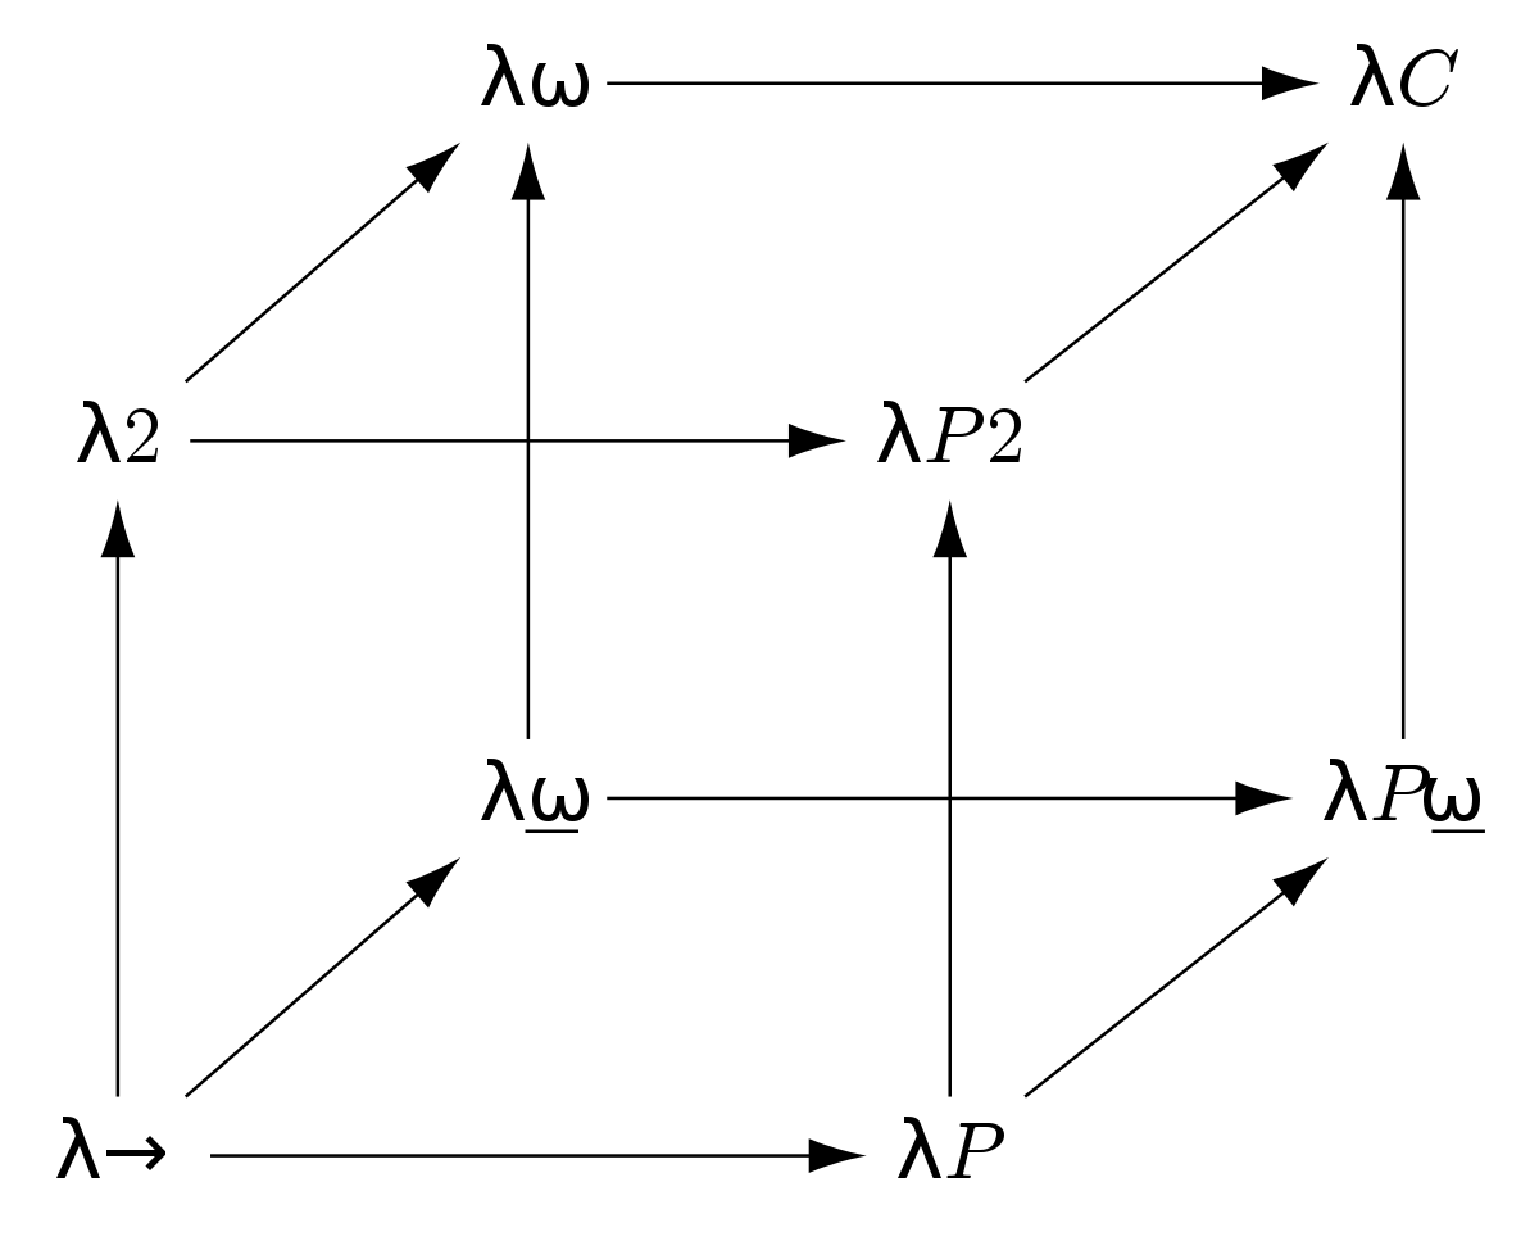
\includegraphics[width=3cm]{1200px-Lambda_Cube_img}
\caption{The lambda cube by Henk Barendregt \cite{lambda_cube}.}
\label{fig:lambda_cube}
\end{figure}

The biggest benefit of dependent types is the possibility to formulate constructive proofs about the desired properties of the program directly in the program itself.
If the need for safe and secure software continues to increase as it did in the past, the need for dependent types will likely increase as well.
It is not realistic that every software developer will use dependent types, however, it can be of great advantage to know dependent types exists as well as the basics of the concept.

As the concept of dependent types directly relates to an extended version of the lambda calculus, most of the currently known implementations are found in functional languages.
In this publication, all code examples are based on Agda, because there are different beginner-friendly tutorials available as well as literature related to dependent types. 
Amogst others this includes "Dependently Typed Programming in Agda" from Ulf Norell \cite{norell:deptyped}, "Programming Languages Foundations in Agda" from Phil Wadler \cite{plfa2019} as well as "Verified Functional Programming in Agda" from Aaron Stump \cite{10.1145/2841316} on which most of the examples are based\footnote{A comprehensive list can be found in the documentation of Agda \cite{AgdaReadTheDocs}.}.

Section \ref{section:first_steps_in_agda} contains an introduction to Agda.
It includes all concepts and definitions required to understand the examples in section \ref{section:dependent_types}.
Section \ref{section:dependent_types} introduces the concept of \emph{Dependent Types}.
Section \ref{section:limits} contains a short summary of limitations that dependent types have together with a few examples where dependent types are currently in use.

Basic knowledge of lambda calculus as well as any functional programming language, such as Haskell, is recommended to benefit the most from the following sections.

\section{First steps in Agda}\label{section:first_steps_in_agda}
In the following chapter, a brief introduction to Agda is given. If you are experienced in any functional programming, it will be a short read or you might even skip some parts.

\subsection{Preliminaries}
Agda is an advanced functional programming language. Its syntax is strongly related to Haskell but it differs concept-wise in some topics. 

One thing to mention is that Agda supports the full Unicode characters in the source code with only a few reserved symbols\footnote{\, . ; \{ \} ( ) @ " are reserved symbols\cite{AgdaReadTheDocsStructure}} 
and some reserved keywords\footnote{A full list of reserved keywords can be found at \cite{AgdaReadTheDocsStructure}}. 
Unicode symbols will be used a lot, especially for mathematical symbols.

Another important thing to mention is the integration into emacs, which works as an IDE and supports syntax highlighting as well as many agda specific features some of which are pointed out in this publication.

\subsection{Introductory example}\label{section:agda_introduction_example}
\subsubsection{Datatype Definitions}
Lets first look at the datatype definition for Peano natural numbers $\mathbb{N}$ shown in code snippet \ref{codeSnippet:natural_number}.

\begin{codesnippet}[mathescape=true, caption={Definition of the peano natural numbers datatype in Agda}, label={codeSnippet:natural_number}]
data $\mathbb{N}$: Set where
  zero : $\mathbb{N}$
  suc  : $\mathbb{N} \rightarrow \mathbb{N}$
\end{codesnippet}

To define a new datatype it is required to specify the name of the type after the keyword \emph{data}.
Separated by a colon the type of the new datatype is defined - normally this is \emph{Set}.
It is required to specify the type of this new datatype because in Agda every expression has a type \cite{10.1145/2841316}.

After this basic definition two different constructors \emph{zero} and \emph{suc} are defined as shown in code snippet \ref{codeSnippet:natural_number}.
There is little meaning in this short definition other than elements constructed with these operations are of type $\mathbb{N}$.
The only additional information is that \emph{suc} requires another $\mathbb{N}$ to be constructed.

Elements of $\mathbb{N}$ can now be constructed by calling the constructors and used in functions with pattern matching. 
Code snippet \ref{codeSnippet:natural_number_constructor} shows the basic usage of the two different constructors.

\begin{codesnippet}[mathescape=true, caption={Some peano numbers}, label={codeSnippet:natural_number_constructor}]
x = zero
y = suc zero
z = suc (suc (suc zero))
\end{codesnippet}

\subsubsection{Type levels}
\emph{Set} is a special kind of type which is the type of types.
But not every type is of type \emph{Set}. 
This would lead to non-terminating behaviour, as the type of \emph{Set} would also be \emph{Set}.

Agda instead uses an infinite number of $Set$ types, $Set_0$, $Set_1$, $Set_2$, ..., where elements of the next Set are potentially larger.
The type $Set_n$ is of type $Set_{(n+1)}$ where $Set_n$ is a \emph{universe} and n is called \emph{universe level} or \emph{type level} \cite{AgdaReadTheDocs, 10.1145/2841316}.
\emph{Set} without any number as used in the definition of $\mathbb{N}$ is just an abbreviation for $Set_0$. 
Each set $Set_n$ can also be expressed as \emph{Set n}, which is very common in definitions.

\subsubsection{Mixfix Operators}
Addition of Peano numbers can be defined in a very elegant way as an infix operator as shown in code snippet \ref{codeSnippet:natural_number_addition}.

\begin{codesnippet}[mathescape=true, caption={Peano numbers addition}, label={codeSnippet:natural_number_addition}]
_+_ : $\mathbb{N} \rightarrow \mathbb{N} \rightarrow \mathbb{N}$
zero  + n = n
suc m + n = suc (m + n)
\end{codesnippet}

Infix operators are functions which can be used in between its arguments in which the underscores determines the place of its arguments.
Alternativelly it is also possible to call these functions in the normal prefix notation, but in this case the underscores are mandatory\footnote{In case of the \_+\_ the infix call is \emph{n + m} and the equivalent prefix call is $\text{\_+\_}$ \emph{n m}}.

Infix operators are a special case of mixfix operators where the operator is in between the arguments.
However, mixfix operators are not restricted to two arguments, but allow more complex constructs such as $\text{if\_then\_else\_}$ \cite{AgdaReadTheDocs}.

To be able to use multiple infix operators in the same expression it is necessary to specify different precedences.
With the three different keywords \emph{infix}, \emph{infixr} and \emph{infixl} the precedence as well as the associativity of the operator can be defined\footnote{The precendence factor defaults to 20 and can also be negative.}.

\begin{codesnippet}[mathescape=true, caption={Precedence and associativity of some Peano number operators}, label={codeSnippet:natural_number_precedence}]
infixl 40 _+_
infixl 20 _<_
\end{codesnippet}

An additional function for Peano numbers which is used in this publication is the comparison function shown in code snippet \ref{codeSnippet:natural_number_less_than}.

\begin{codesnippet}[mathescape=true, caption={Peano numbers less-than}, label={codeSnippet:natural_number_less_than}]
_<_ : $\mathbb{N} \rightarrow \mathbb{N} \rightarrow \mathbb{B}$
0 < 0 = false
0 < (suc y) = true
(suc x) < (suc y) = x < y
(suc x) < 0 = false
\end{codesnippet}

The \_\textless\_ function follows the same structure as the \_+\_ function, but includes four different pattern matching cases. 
This might not be the smallest possible definition possible but it is very precise and comprehensible.

The boolean datatype $\mathbb{B}$ consists of two constructors \emph{true} and \emph{false} and is shown in code snippet \ref{codeSnippet:boolean} for completeness.

\begin{codesnippet}[mathescape=true, caption={Definition of the boolean datatype in Agda}, label={codeSnippet:boolean}]
data $\mathbb{B}$ : Set where
  true : $\mathbb{B}$
  false  : $\mathbb{B}$
\end{codesnippet}

\subsubsection{Type Parameters}
The definition of the list datatype as seen in code snippet \ref{codeSnippet:list_datatype} is more complex than the previous datatype definitions of $\mathbb{B}$ and $\mathbb{N}$ as it contains the type parameter \emph{A}.
The application of another type to the list datatype results in an own unique type.

\begin{codesnippet}[mathescape=true, caption={Definition of the list datatype in Agda}, label={codeSnippet:list_datatype}]
data $\mathbb{L}$ {$\ell$} (A : Set $\ell$) : Set $\ell$ where
  [] : $\mathbb{L}$ A
  _::_ : (x : A) (xs: $\mathbb{L}$ A) $\rightarrow \mathbb{L}$ A
\end{codesnippet}

In this specific example, to construct a new list, the input is type \emph{A} of type level $\ell$  is required. For example $\mathbb{L}$ $\mathbb{N}$ for the list of Peano numbers.
The newly constructed type $\mathbb{L}$ \emph{A} will be at the same type level $\ell$.

$\ell$ is just an additional argument, but the curly braces around $\ell$ indicate, that it is an implicit argument and should be inferred by Agda.
There is no guarantee that the type checker is able to infer implicit arguments and it fails otherwise.
However, it is always possible to specify the implicit arguments in the call by enclosing the argument in curly braces\cite{norell:deptyped}.

If $\ell$ is omitted from the type definition of $\mathbb{L}$, it is no longer be possible to construct a list type for higher universe types.
Suppose a list of types \emph{$\mathbb{B}$ :: []}. 
The type of this expression is \emph{$\mathbb{L}$ Set} and therefore the type parameter \emph{A} is \emph{Set}. 
Because \emph{Set} itself is of type $Set_1$ the definition without $\ell$ would not allow this usage.

\todo{maybe note that the type parameter must be equal in the return type of all constructors}
When a parameter in a datatype definition is declared it can be used in the types of the constructors.
For example, the second constructor is defined as a function that takes an argument \emph{x} of type \emph{A} and a second argument \emph{xs} of type $\mathbb{L}$ \emph{A} and returns a new $\mathbb{L}$ \emph{A}, where \emph{A} is exactly the type that was used to construct the type of the list.

With the help of the two constructors, it is possible to construct any possible list. 
The next function to consider is $\text{\_++\_}$, which appends two lists of the same type, shown in code snippet \ref{codeSnippet:list_append}. 
In combination with the examples in chapter \ref{section:dependent_types}, this example will help to understand the difference between generic and dependent types.

\begin{codesnippet}[mathescape=true, caption={Definition of the list append function in Agda}, label={codeSnippet:list_append}]
_++_ : $\forall$ {$\ell$} {A : Set $\ell$} $\rightarrow \mathbb{L}$ A $\rightarrow \mathbb{L}$ A $\rightarrow \mathbb{L}$ A
  []        ++ ys = ys
  (x :: xs) ++ ys = x :: (xs ++ ys)
\end{codesnippet}

To call this function, two implicit and two explicit arguments are required. 
Agda infers the correct type-level $\ell$ and the type \emph{A} from the explicit arguments of type $\mathbb{L}$ \emph{A}. 
It is required that both input arguments are of the same type $\mathbb{L}$ \emph{A}, and therefore it is possible to infer that the return value is also of type $\mathbb{L}$ \emph{A}.

The second function for lists, that is of interest, is \emph{nth} which returns the element at the specified position of a list.
In particular, the comparison with the same function for vectors, which is shown in chapter \ref{section_dependent_types_example}, can help to understand dependent types.

One fundamental problem of the access to a specific position has, is that the list might not be long enough.
In many common programming languages, this results in an exception. However, the concept of exceptions is not included in Agda, to maintain the properties of a total language.
A more detailed explanation can be found in section \ref{section:total_languages}.

To overcome this issue, an additional datatype \emph{maybe} is introduced\footnote{In other languages, such as Java, the concept of the \emph{maybe} datatype is known as \emph{Optional}}.
This datatype is either a wrapper around another element or indicates the absence of it.

\begin{codesnippet}[mathescape=true, caption={Definition of the maybe datatype in Agda}, label={codeSnippet:maybe_datatype}]
data maybe {$\ell$} (A : Set $\ell$) : Set $\ell$ where
  just : A $\rightarrow$ maybe A
  nothing : maybe A
\end{codesnippet}

The function \emph{nth} as shown in code snippet \ref{codeSnippet:list_nth} takes two implicit arguments for the type level and the type \emph{A} itself.

\begin{codesnippet}[mathescape=true, caption={Definition of nth function in Agda}, label={codeSnippet:list_nth}]
nth : $\forall$ {$\ell$} {A : Set $\ell$} $\rightarrow \mathbb{N}$ $\rightarrow \mathbb{L}$ A $\rightarrow$ maybe A
nth _ [] = nothing
nth 0 (x :: xs) = just x
nth (suc n) (x :: xs) = nth n xs
\end{codesnippet}

In addition to the implicit arguments, the index of the desired element of type $\mathbb{N}$, as well as the list itself, have to be specified.

The \emph{maybe} datatype solves the discussed issue for the function \emph{nth}, but wherever the \emph{nth} function is used, a case distinction is required to handle the \emph{nothing} case.

\subsection{Total languages}\label{section:total_languages}
In comparison to other programming language, Agda is a so-called total programming language \cite{AgdaReadTheDocs}.
This means that every valid Agda programs will always terminate with the correct type. There is no exception to this.

In contrast to this, non-total languages often terminate with the correct type. 
But they may also raise an exception because something was not as expected and the behaviour for this special case was not defined, or not terminate at all.

It is fundamental for Agda to be total because computations can be already required during type checking.
If non-terminating computations were possible, type checking itself would be undecidable\cite{agda_wiki_totality}.

To ensure the totality of a program beside type checking, coverage checking as well as termiantion checking are of great importance. 
Additionally \emph{strict positivity of constructors} as well as \emph{guardedness in coinductive programs} have to be checked, which are not discussed further in this publication.

Coverage checking verifies that no partial function is defined. A partial function is a function with pattern matching that does not cover all cases.
As opposed to Haskell, where partial functions are compiled successfully and only throw an exception when a not covered case is required at runtime, Agda does not compile partial functions.

To be able to check a program for termination Agda accepts only two different recursive schemas which can be proven to terminate.

In the case of \emph{primitive recursion} the recursive call must be executed with an argument that is exactly one constructor smaller than in the original call.

For example in the addition of Peano Number in code snippet \ref{codeSnippet:natural_number_addition} the arguments used in the recusive call have to be structurally smaller \cite{norell:deptyped}. 
This is the case as $m$ is structurally smaller than \emph{suc m} based on the definitions of the $\mathbb{N}$ datatype.

Beside \emph{primitive recursion} Agda is able to determine termination on \emph{structural recursion}.
This requires the argument of the recursive call to be a subexpression of the original argument.
As a contrast to \emph{primitive recursion} a recusive call with $m$ is also possible if the original argument was \emph{suc(suc m)}.
\section{Dependent Types}
\subsection{Introduction to dependent types}
There are different kinds of dependent types. The two most common ones are $\Sigma$-types and $\Pi$-types.
The first focus lies on the $\Pi$-types, which are also used in the first example in section \ref{section_dependent_types_example}. These types are sometimes also called \emph{dependent function types} as in \cite{10.1145/2841316} or \emph{dependent product type} as in \cite{10.5555/1076265}. Be aware that the name dependent product type can also be used for $\Sigma$-types as in \cite{10.1145/2841316}.

In the introduction in section \ref{section:introduction} the concept of an enhanced list, where the length is a part of the type, was introduced.
This data structure is in the literature often called vector \cite{10.1145/2841316} \cite{10.5555/1076265}.
This new data structure is not a simple type but maps an input of type \emph{Nat} to a specific type. To differentiate between such as structure and types the term \emph{type family} is used as suggested by Aspinall and Hofmann in \cite{10.5555/1076265}.

$$Vector :: Nat \rightarrow *$$

The type which contains vectors of length \emph{k} can be constructed by applying \emph{k} to \emph{Vector} or in other terms \emph{Vector k}.

To construct new Vectors two constructors are needed. 
One which constructs an empty vector and one to add new elements to the vector. 
This pattern should be familiar for everyone that is used to functional programming so far.

The second constructor \emph{cons} takes one element \emph{n} of type \emph{Nat}, an element of type \emph{data} as well as a vector with the length \emph{n} and returns a new vector of length \emph{n+1}. 
The length of the returned vector is increased by one to account for the new element that is added.

$$empty: Vector \, 0$$
$$cons : \Pi n : Nat. \, data \rightarrow Vector \, n \rightarrow Vector \, (n+1)$$

Dependent function types can be described as $\Pi x : A. B$ where x can be used to define B. 
This is the generalization of the arrow type used in simply typed lambda-calculus. Every arrow type can also be expressed as a $\Pi$-type.

\todo{Verify}
$$A \rightarrow B \, = \, \Pi x:A.B$$
$$where \, x \, does \, not \, appear \, free \, in \, B$$

Another description of the $\Pi$-type is the following. A function maps an element $a \in A$ to a new element $b \in B_a$. 
This is also called type B is indexed by type A \cite{10.1145/2841316}.

\todo{Extend this with relation to Curry-Howard Isomorphism/Correspondence as universal quantification}

This additional information that is now encoded in the type can be exploited whenever such a type is used. 
Consider a first example, where the function \emph{head} is defined, which returns the first element of a vector.

$$head : \Pi n : Nat.Vector(n+1) \rightarrow data$$

In contradiction to lists, it is now possible to specify that only non-empty vectors can be be used as an argument. 
This is archived by specifying an type variable \emph{n} of type \emph{Nat} and only accepting vectors of length \emph{n+1}.
As the smallest possible natural number is 0, vectors of length 1 are the smallest accepted vectors.

This simplifies the implementation of \emph{head} and also each usage of \emph{head} as no exception handling for the empty data structure is necessary. 
If the function can be called with a specific instance then it is guaranteed by the type system that an instance of data is returned.


To be more clear what this means in practice lets consider a few examples in Agda.

\subsection{$\Pi$-Types in Agda}\label{section_dependent_types_example}
In this section, the first dependent datatype in Agda, the vector, will be defined.

It is essentially a list but in contrast to the list datatype defined in section \ref{section:agda_introduction_example} the length of the list is a part of the type.

In addition to the implicit type-level and the type A, an additional parameter of type $\mathbb{N}$ is defined in the type definition as shown in code snippet \ref{codeSnippet:vector_datatype}.

\begin{codesnippet}[mathescape=true, caption={Definition of the vector datatype in Agda}, label={codeSnippet:vector_datatype}]
data $\mathbb{V}$ {$\ell$} (A : Set $\ell$) : $\mathbb{N}$ $\rightarrow$ Set $\ell$ where
  [] : $\mathbb{V}$ A zero
  _::_ : {n : $\mathbb{N}$} (x : A) (xs: $\mathbb{V}$ A n) $\rightarrow$
         $\mathbb{V}$ A (suc n)
\end{codesnippet}

There is a difference between \emph{parameters}, used before the colon, and \emph{indices} of a datatype.
The datatype $\mathbb{V}$ is parameterised by a type A and indexed over $\mathbb{N}$\cite{norell:deptyped}.
Parameters are required to be exactly the same for each constructor of a datatype, however, indicies can vary.

The first constructor for the empty vector sets the length of the vector to the fixed value zero of $\mathbb{N}$ because it is known that the list is currently empty and the length is therefore 0.
The second constructor is used to add new elements to an existing vector. It takes two arguments one of type A and one of type $\mathbb{V}$ A n similar to the list but additionally it determines the implicit argument n of type $\mathbb{N}$ from the input vector.
This parameter is then used to define the return type. As exactly one new element is added to the existing list of type $\mathbb{V}$ A n it is known that the new type has to be $\mathbb{V}$ A (suc n).

Appending two vectors - as seen in code snippet \ref{codeSnippet:vector_append} - is a mix between the appending of two lists and the datatype definition of the vector and relatively straightforward.

\begin{codesnippet}[mathescape=true, caption={Definition of the vector append function in Agda}, label={codeSnippet:vector_append}]
_++$\mathbb{V}$_ : $\forall$ {$\ell$} {A : Set $\ell$}  {n m: $\mathbb{N}$ $\rightarrow$
        $\mathbb{V}$ A n $\rightarrow \mathbb{V}$ A m $\rightarrow \mathbb{V}$ A (n + m)
  []        ++$\mathbb{V}$ ys = ys
  (x :: xs) ++$\mathbb{V}$ ys = x :: (xs ++$\mathbb{V}$ ys)
\end{codesnippet}

To prevent a naming conflict between the append operators of lists and vectors the unique name \_++$\mathbb{V}$\_ was chosen.

It is important, that the types of these two vectors does not need to be equal, as the parameters n and m of type $\mathbb{N}$, which are also a part of the types, can have different values. 
Nevertheless the elements contained in both vectors are still required to be of type A.

It can be deduced that the newly constructed vector has the type $\mathbb{V}$ A (n + m).

The next example will present the first benefit of including the length in the datatype.
In case of the list datatype $\mathbb{L}$, it was required to define an additional helper datatype \emph{maybe} as described in section \ref{section:agda_introduction_example} when implementing the \emph{nth} function.
Additionally, whenever a programmer uses the function, he has to think of the different cases \emph{nothing} or \emph{just} and adjust his functionality. This is done with additional pattern matching.

The same restrictions are met by the \emph{head} function of a $\mathbb{L}$. 
However, the \emph{head} function of $\mathbb{V}$ shown in code snippet \ref{codeSnippet:vector_head} always returns a single object of type A.

\begin{codesnippet}[mathescape=true, caption={Definition of $head\mathbb{V}$ function in Agda}, label={codeSnippet:vector_head}]
head$\mathbb{V}$ : $\forall$ {$\ell$} {A : Set $\ell$} {n : $\mathbb{N}$} $\rightarrow$ 
        $\mathbb{V}$ A suc(n) $\rightarrow$ A
head$\mathbb{V}$ (x :: _) = x
\end{codesnippet}

This is possible by using the additional information of the implicit parameter \emph{n} of type $\mathbb{N}$, respectivelly by restricting the input vector to the type $\mathbb{V}$ A suc(n).
Elements of this type are known to have a least one entry, in this case the implicit parameter would be zero.

It is possible to define the \emph{head} without specificing a pattern for the empty vector [] as the type checker can infer that this case is not possible.
Whenever a particular case is type correct it is necessary to include it, otherwise it needs to be omitted \cite{norell:deptyped}.

\subsection{Proofs as programs}\label{section:agda_proofs}
\todo{Maybe move this (or parts of it), as in some proofs such as x+0 dependent function types are used before they are introduced.}
In this section a small introduction to \emph{Propositions as Types}\cite{10.1145/2699407} will be given together with a few examples in Agda. \emph{Proposition as Types} is also known under the names \emph{Curry-Howard Correspondence}\cite{10.5555/1076265} and \emph{Curry-Howard Isomorphism}\cite{10.1145/2841316} and many more.

Under all this different names the same interlinking between logic and programming is understood. There are three main statements of interest, pointed out by Wadler in \cite{10.1145/2699407}.

\emph{Propositions as types} states that each proposition in a logic has a corresponding type in the programming world and the other way around. 

\emph{Proofs as programs} follows from the fact that each proof is mapped to its proposition, as well as each program has its own type.

\emph{Simplification of proofs as evaluation of programs} states that for every step in simplification of a proof there is an operation how to evaluate the corresponding program.

This allows it that proofs can be directly represented in the programming language.

\subsubsection{Proofs as programs in Agda}
Lets now consider a first small example in Agda.

In Agda it is possbile to define propositional equalities such as $zero + suc(zero) \equiv suc(zero)$. The type of this term is \emph{Set} which is the type of types. This was the first application of propositions as types.
However this proposition is not proved yet. It is also possible to state false propositions such as $zero + suc(zero) \equiv zero$ without any compiler errors.

To prove this proposition a program of the type $zero + suc(zero) \equiv suc(zero)$ has to be implemented.
As a start a useful name has to be considered. Agda is very liberal in terms of naming and even the previously defined operators can be used to define names. Possible examples for name of the proof include $\text{1+0=1}$ or $zeroAddition$.

$$\text{0+1=1} : zero + suc(zero) \equiv suc(zero)$$

Agda is able to simplify this type to $suc(zero) \equiv suc(zero)$ because $suc(zero) + zero$ is definitionally equal to $suc(zero)$. Definitionally equal means that Agda is able to simplify both terms to the same value and they are therefore interchangable.
The proof is simple as both sides are equal. 
Agda needs the hint by using the value $refl$, which means reflexivity and requires both sides of the $\equiv$ operator to be definitionally equal.

$$\text{0+1=1} = refl$$

If the program gets typechecked successfully, the proof is completed.

This proof is very specific to these values, similiar to a single test case. But it is possible to extend this proof to any Peano number $\mathbb{N}$. 
To do this the universal quantifier $\forall$, which is also common in mathematics, is used. It allows it to state that the following property should hold for every possible assignment\cite{plfa2019}.
The $\forall$ symbol is one of the few reserved keywords in Agda.

The new proposition in code snippet \ref{codeSnippet:zero_plus_x_agda} is now a little more complex but still comprehensible. It states that for every x of type $\mathbb{N}$ the following equivalence holds. 
Because an variable \emph{x} is defined in the type, the program requires an input argument. In this code snippet this argument gets assigned to the variable \emph{a}.

\begin{codesnippet}[mathescape=true, caption={Proof of addition to zero in Agda}, label={codeSnippet:zero_plus_x_agda}]
0+x : $\forall$ (x : $\mathbb{N}$) $\rightarrow$ zero + x $\equiv$ x
0+x a = refl
\end{codesnippet}

As the first constructor of the addition of $\mathbb{N}$ is $zero + n = n$ refl is the proof.

If the addition happens in a different order and \emph{zero} gets added to \emph{x}, as shown in code snippet \ref{codeSnippet:x_plus_zero_agda}, the proof gets yet a little bit more complicated. 
The reason for this lies in the definition of addition.
Because the recursion happens on the second argument it is no longer possible for Agda to determine that these terms are definitionally equal and requires the programmer to add additional hints to be able to prove the equality.

\begin{codesnippet}[mathescape=true, caption={Proof of addition of zero in Agda}, label={codeSnippet:x_plus_zero_agda}]
x+0 : $\forall$ (x : $\mathbb{N}$) $\rightarrow$ x + zero $\equiv$ x
x+0 zero = refl
x+0 suc(a) rewrite x+0 a = refl
\end{codesnippet}

As shown in code snippet \ref{codeSnippet:x_plus_zero_agda} it is possible to pattern match in proofs as proofs are programms.
For the base case \emph{zero + zero $\equiv$ zero}, \emph{refl} is still enough but on the case where \emph{a} is not \emph{zero} but \emph{suc(x)}, the \emph{rewrite} directive is required.

The \emph{rewrite} directive can be used to transform parts of the original problem. If a proof A $\equiv$ B exists, then \emph{rewrite} will replace A with B in the instantiated type.

But how does this really work?
The original proof is $x + zero \equiv x$ where x is instantiated with \emph{suc(a)} or more precisely $suc(a) + zero \equiv suc(a)$.
As $suc(a) + zero$ is definitionally equal to $suc(a + zero)$ regarding the second constructor of addition in code snippet \ref{codeSnippet:natural_number_addition}, this can also be written as $suc(a + zero) \equiv suc(a)$.

If the proof that $a + 0 \equiv a$ gets applied to this, the result will be the desired $suc(a) \equiv suc(a)$. 
To get the proof $a + 0 \equiv a$ \emph{x+0} gets called recursively on $a$ instead of $suc(a)$

This kind of proof is called proof by induction in mathematics and is actually very common.
The important thing to remember, as in every recursion, is that a base case as well as partial solution step are required.

\subsubsection{Proofs as arguments}

Similar to \emph{head$\mathbb{V}$} the function \emph{nth$\mathbb{V}$} in code snippet \ref{codeSnippet:vector_nth} has an implicit parameter m of type $\mathbb{N}$ which represents the length of the input vector. 
However, it contains an additional explicit parameter, which is a proof that n is less than m.

\begin{codesnippet}[mathescape=true, caption={Definition of \emph{nth} function in Agda}, label={codeSnippet:vector_nth}]
nth$\mathbb{V}$ : $\forall$ {$\ell$} {A : Set $\ell$} {m : $\mathbb{N}$} $\rightarrow$
       (n : $\mathbb{N}$) $\rightarrow$ n < m $\equiv$ tt $\rightarrow \mathbb{V}$ A m $\rightarrow$ A
nth$\mathbb{V}$ zero _ (x :: _) = x
nth$\mathbb{V}$ (suc n) p (_ :: xs) = nth$\mathbb{V}$ n p xs
nth$\mathbb{V}$ (suc n) () []
nth$\mathbb{V}$ zero () []
\end{codesnippet}

The base case of the \emph{nth$\mathbb{V}$} recursive function is at line 3. It states that if the element at index 0 is wanted, the head of the list is returned.
To indicate that the proof, that zero is smaller than length of the vector, as well as the tail of the vector are not used in the definition of the function they are replaced by an \_.

At line 4 the recursive case is defined which calls \emph{nth$\mathbb{V}$} but with the predecessor of n and the tail of the current vector.
The second argument \emph{p}, which contains the proof that $suc(n)$ is smaller than the length of the vector, is directly passed into the new function call. 
At first glance, this might look a little bit unusual. 
It is possible because, both the index as well as the length of the new vector \emph{xs} are decreased by exactly one, the proof still holds.
The proof \emph{p} is still valid as \emph{suc n $<$ suc m $\equiv$ tt} and \emph{n $<$ m $\equiv$ tt} are definitionally equal.

The last two lines look quite different than any of the definitions before.
Because it is not possible to prove that \emph{suc n $<$ m $\equiv$ tt} where m is the length of the empty list, or more concretely zero, the so-called absurd pattern can be used. 
This basically tells Agda that this case can never be reached and therefore no definition for this case has to exist.
The last line is required lies in the definition of \_$<$\_ of $\mathbb{N}$ shown in code snippet \ref{codeSnippet:natural_number_less_than}.
Because in that definition a case distinction between $0 < 0$ and $\text{(suc x)} < 0$ was made, the last line, which proves that \emph{zero $<$ zero $\equiv$ tt} is false, is required as well.

Whenever the function \emph{nth$\mathbb{V}$} is called, a proof that m $<$ n is equivalent to tt is required as shown in code snippet \ref{codeSnippet:vector_nth_usage}. This can easily be done by using refl.

\todo{state that a digit representation is possible without going into details about pragmas. Maybe in the agda section.}
\begin{codesnippet}[mathescape=true, caption={Usage of \emph{nth} function in Agda}, label={codeSnippet:vector_nth_usage}]
testVector = ff :: ff :: []
element = nth$\mathbb{V}$ (suc zero) refl testVector

invalid_element = nth$\mathbb{V}$ (suc(suc zero)) 
                  refl testVector
\end{codesnippet}

The code snippet \ref{codeSnippet:vector_nth_usage} will not compile, as the proof refl in the call on the last line is invalid, as \emph{suc(suc zero) $<$ suc(suc zero) $\equiv$ ff}.

\subsection{$\Sigma$-types}
In addition to $\Pi$-types, there exists a second important class of dependent types. 
The $\Sigma$-types also called \emph{dependent product types}\cite{10.1145/2841316},\emph{dependent pair types}\cite{10.1145/2841316} or \emph{dependent sum types}\cite{10.5555/1076265}.

A $\Sigma$-type is the generalization of the ordinary product type. 
It is basically a combination of two types where each element of this type is a pair. 
But the type of the second element of the pair may depend on the value of the first element.

\todo{Verify}
$$\Sigma x: A.B \,= \, A \times B$$
$$where \, x \, does \, not \, appear \, free \, in \, B$$


Another good description of the $\Sigma$-type is the following. 
Elements of the type are pairs $(a, b)$ under the condition that $a \in A$ and $b \in B_a$.

\todo{Extend this with relation to Curry-Howard Isomorphism/Correspondence as existential quantification}
Dependent $\Sigma$-types are often used to express an element with a certain property and its corresponding proof.
\todo{maybe add an example}

\subsection{$\Sigma$-types in Agda}
The simplest example for $\Sigma$-types in Agda is the type of nonzero Peano numbers.
It is directly based on the Peano numbers $\mathbb{N}$ defined in section \ref{section:agda_introduction_example}.

The definition of $\mathbb{N}^+$ states that each element is a pair of a Peano number combined with the proof that this specific number applied to the \emph{iszero} function returns false.

\begin{codesnippet}[mathescape=true, caption={Definition of nonzero Peano numbers in Agda}, label={codeSnippet:nonzero_natural_number}]
$\mathbb{N}^+$ : Set
$\mathbb{N}^+$ = $\Sigma$ $\mathbb{N}$ ($\lambda$ n $\rightarrow$ iszero n $\equiv$ ff)
\end{codesnippet}

The $\Sigma$ used in code snippet \ref{codeSnippet:nonzero_natural_number} from IAL is a simplification of the one defined in the standard library of Agda and only consists of three lines shown in code snippet \ref{codeSnippet:sigma}.

The $\Sigma$ type constructor takes two explicit and two implicit arguments. 
The first type argument is the type A of level $\ell$, the second type argument is a function of type B which takes an element of A and returns a new type of level $\ell '$.
The type level of $\Sigma$ will be at $\ell$ $\sqcup$ $\ell '$. The operator $\sqcup$ is part of Agda's primitive level system and takes the maximum of the two input levels.

The constructor for new elements of type $\Sigma$ is a single comma, which allows it to express $\Sigma$ elements as pairs.
The  usage of the variable a of type A in the type definition of b shows the direct dependence of the second component to the value of the first component.

\begin{codesnippet}[mathescape=true, caption={Definition of $\Sigma$ in Agda}, label={codeSnippet:sigma}]
data $\Sigma$ {$\ell$ $\ell '$} (A : Set $\ell$) (B : A $\rightarrow$ Set $\ell '$)
 : Set ($\ell$ $\sqcup$ $\ell '$) where
_,_ : (a : A) $\rightarrow$ (b : B a) $\rightarrow$ $\Sigma$ A B
\end{codesnippet}

Code snippet \ref{codeSnippet:nonzero_natural_number_suc} contains the successor function of $\mathbb{N}^+$ which returns the next nonzero Peano number.
As an input argument, the function takes an element of $\mathbb{N}^+$ and returns a new element $\mathbb{N}^+$. 
With pattern matching the element of $\mathbb{N}^+$ is disassembled into the number x and the proof p as defined in code snippet \ref{codeSnippet:nonzero_natural_number}.

The return value is constructed by applying the function \emph{suc} to the variable x as the first part of the pair and the \emph{refl} proof as the second part of the pair.
Agda can prove that \emph{iszero (suc x)} is always false and therefore the proof is as simple as refl.

\begin{codesnippet}[mathescape=true, caption={Successor of $\mathbb{N}^+$}, label={codeSnippet:nonzero_natural_number_suc}]
suc$^+$ : $\mathbb{N}^+$ $\rightarrow$ $\mathbb{N}^+$
suc$^+$ (x, p) = (suc x, refl)
\end{codesnippet}
\section{Internal versus external verification}
Highlight the differences between external and internal verification and give some examples where which should be prefered.

\section{Theoretical and practical limits}\label{section:limits}
\subsection{Theoretical limits}
As already discussed in section \ref{section:total_languages} dependent types require a total language to be able to represent programs as proofs.
This also requires recursive functions to be in a special scheme.
Currently, only simple recursions are supported in popular dependently typed languages such as Agda, but more powerful termination-checkers are under research.

In Agda it is possible to disable termination checking with the consequence that certain properties can not be proved.
\subsection{Practical limits}
In addition to the theoretical limits that languages that support dependent types have, there are additional problems for the use of dependent types in practical software.
The most important limitation is that writing proofs, which is one of the main features that dependent types enable, can be extremely difficult and time-consuming.
Aaron Stump gives the following statement in Verified Functional Programming in Agda \cite{10.1145/2841316}:
\begin{quote}
Yes, mathematicians are in business for a reason: theorem proving can be extremely difficult, with a single conjecture stumping the brightest minds humankind has to offer for centuries.
\end{quote}

Another obstacle is that some functions, which are actually terminating, are not directly recognised as structurally terminating which increases the implementation effort enormously.
The most common example is the division function of Peano numbers $\mathbb{N}$, which replicates the Haskell \emph{div} function from code snippet \ref{codeSnippet:division}.
There are two problems when implementing such as function in Agda. The minor is that the proof that m is not zero has to be included, the second is that \emph{m - n} is not recognised as structurally smaller than \emph{m}. Both of these problems can be solved but the resulting function is complex.
\begin{codesnippet}[mathescape=true, caption={Definition of div function in Haskell}, label={codeSnippet:division}]
div m n | m < n = 0
div m n | m >= n = 1 + div (m - n) n
\end{codesnippet}

The division example and its solution is contained in an own chapter in different publications \cite{10.1145/2841316, Bove2009} but will not be discussed further in this publication.

\subsection{Who and where to use}
This publication is heavily focused on Agda but there are many other languages which support dependent types and some of them are more common in the industry.
Even though Agda programs can be compiled to Haskell or JavaScript there are little references found that use Agda to solve practical problems but only used as an introduction to programming language theory or the concept of dependent types.

In 2016 Eisenberg wrote in \emph{Dependent Types in Haskell: Theory and Practice} \cite{DBLP:journals/corr/Eisenberg16}: 
\begin{quote}
Haskell, as implemented in the Glasgow Haskell Compiler (GHC), has been adding new type-level programming features for some time. Many of these features---chiefly: generalized algebraic datatypes (GADTs), type families, kind polymorphism, and promoted datatypes---have brought Haskell to the doorstep of dependent types. Many dependently typed programs can even currently be encoded, but often the constructions are painful.
\end{quote}

In the same publication, he introduced additional support for dependent types directly into GHC. It is currently listed as a proposal to extend Haskell with dependent types in the Haskell wiki \cite{haskell_wiki}.

Even though there are efforts to improve the situation for Haskell, and with it introduce dependent types to a much bigger community, it seems that it has not improved very much in the last years.

A case analysis from Christiansen et al \cite{10.1145/3341704} on the construction of a Haskell library for symbolic execution, which uses dependent type features, shows that the new features allowed to improve the code correctness. The static well-formedness checks, which could be introduced, helped during refactorings as well. However, they noticed different difficulties, including tooling support, type system limitations, as well as the massive need for manual proofs. Additionally, they state that it is hard to find developers who are skilled enough in Haskell and dependently typed programming and that the entry into this combination is laborious.

Another dependently typed programming language that is used in somewhat industry near projects is F*. 
Its most notable usage is in the Project Everest \cite{project_everest_github_io}. The primary aim of Project Everest is to build a fully verified HTTPS stack.
It is mainly driven by Microsoft Researchers in collaboration with different universities and uses F* for many different parts.
Project Everest started in 2016 and is still work in progress, but some parts of it such as verified cryptographic functions are used in productive applications such as the Mozilla Network Security Services\cite{project_everest_slides},  in the WireGuard VPN and others.

\section{Conclusion}
In this publication a short overview of dependent types and its usages in the concept of indexed datatypes as well as constructive proofs have been discussed.

As mentioned already in the introduction, its not realistic, if not illusory, that every software developer uses dependent types. 
They come at a heavy price as it either makes type checking undecidable or restrict the possible programs, as seen at the example of Agda.
Additionally proving properties about a program can take huge amounts of effort and take a lot of practice.
It is uncertain if many developers and companies are willing to invest this effort and profit of the additional safety that dependent types bring.

However, there certainly exists software\footnote{For example the Project Everest\cite{project_everest_github_io}}, where the benefits outweight the costs 


This section contain the conclusion about this paper, especially about dependent types. 
Additionally, I wan't to state my own opinion on how this language feature could be used in practice.
\bibliographystyle{plain}
\bibliography{seminarreferences}

\end{document}